\documentclass[11pt]{amsart}
\usepackage[a4paper,margin=1in]{geometry}
\usepackage{amssymb}
\usepackage{booktabs}
\usepackage{tikz}
\usepackage[font=small,labelfont=bf]{caption}
\usepackage[hidelinks]{hyperref}

\colorlet{copper}{orange!75!black}
\colorlet{inkmuted}{black!60}

\newtheorem{theorem}{Theorem}
\newtheorem{lemma}[theorem]{Lemma}
\newtheorem{proposition}[theorem]{Proposition}
\theoremstyle{remark}
\newtheorem{remark}[theorem]{Remark}

\title{Coins in a Tray}
\author{Vamshi Jandhyala}
\address{London, United Kingdom}
\email{vamshi.jandhyala@gmail.com}

\begin{document}

\begin{abstract}
For which $n$ can coins of radii $\frac12,\frac13,\dots,\frac1n$, at least one of each, be held rigidly in a circular tray of radius~$1$? The asker found arrangements for $n=2,3,4$ and conjectured that there are none for $n\ge5$. We settle two natural special cases. There is no rigid arrangement with every coin on the rim for any $5\le n\le1000$, and none whose contact graph is a triangulation for any $5\le n\le16$. The rim case reduces to deciding which integer relations hold among the angles $\alpha_d=2\arcsin(1/\sqrt d)$ and $\pi$; we decide them exactly with prime-ideal valuations in imaginary quadratic fields, following Conway, Radin and Sadun. For $n=5$ the rim case needs no computer. We also show that no coin $\frac1k$ with $k\equiv0,1,4,5,7,8,9,10,12,13,16,17,19,20,21,22\pmod{24}$ can touch the tray and two coins that touch each other and the tray. The general case remains open.
\end{abstract}

\maketitle

\section{The question}

Dan asked on Mathematics Stack Exchange in June 2024 and on MathOverflow in July 2026~\cite{MO} for which $n$ coins of radii $\frac12,\frac13,\dots,\frac1n$, with at least one coin of each size and no others, can be held rigidly in a circular tray of radius~$1$: no coin can move, except by spinning about its own centre or by all coins turning together about the centre of the tray. He found arrangements for $n=2$ (two half coins), $n=3$ (a half and four thirds) and $n=4$, a ring $\frac13,\frac12,\frac14,\frac14,\frac12$ around the rim (Figure~\ref{fig:rim}(b)), and conjectured that $n\ge5$ is impossible. Before reading on, try to place a $\frac15$ coin on the rim next to the coins of the $n=4$ ring.

Two answers made progress. Matthew House~\cite{House} ran randomised searches for $5\le n\le10$ and found no rigid arrangement, only near-misses with gaps of $10^{-7}$ to $10^{-9}$. The second answer~\cite{U}, by an anonymous user, treated the case where every coin touches the tray and reduced it to the question: which integer relations hold among $\pi$ and the angles $\alpha_d$ below? This note answers that question and draws three consequences.

\begin{theorem}\label{thm:rim}
For $5\le n\le1000$ there is no rigid arrangement in which every coin touches the tray. For $n=5$ the proof is a short argument by hand.
\end{theorem}

\begin{theorem}\label{thm:tri}
For $5\le n\le16$ there is no arrangement, rigid or not, whose contact graph, with the tray as a vertex, is a triangulation.
\end{theorem}

\begin{proposition}\label{prop:desc}
If a coin of radius $\frac1k$ touches the tray and two coins that touch each other and the tray, then $k\equiv2,3,6,11,14,15,18,23\pmod{24}$.
\end{proposition}

The asker's $n=4$ ring is not a triangulation: it leaves a gap with four sides. So the cases left open mix rim coins, interior coins and gaps that are not triangles.

\section{Rim arrangements}

Two coins $\frac1j$, $\frac1k$ that touch the tray and each other have centres at distances $1-\frac1j$ and $1-\frac1k$ from the centre of the tray and $\frac1j+\frac1k$ from each other. The law of cosines gives the angle $\alpha_d$ between them at the centre:
\begin{equation}\label{eq:alpha}
\cos\alpha_d=1-\frac2d,\qquad\text{equivalently}\quad\sin\frac{\alpha_d}2=\frac1{\sqrt d},\qquad d=(j-1)(k-1).
\end{equation}
For example $\alpha_1=\pi$ (two half coins), $\alpha_2=\pi/2$, $\alpha_4=\pi/3$, and $\alpha_3=\arccos\frac13$ for the pair $\frac12,\frac14$ (Figure~\ref{fig:rim}(a)).

If every coin touches the tray, sort the coins by angle. The answer~\cite{U} shows that angularly adjacent coins must touch, since otherwise some coin is held only by the tray and one neighbour, on one side, and slides. So a rim arrangement is a cyclic sequence $\frac1{j_1},\dots,\frac1{j_m}$ using every size, with
\begin{equation}\label{eq:sum}
\sum_{i=1}^m\alpha_{d_i}=2\pi,\qquad d_i=(j_i-1)(j_{i+1}-1),
\end{equation}
and no two coins overlapping. The asker's ring satisfies~\eqref{eq:sum} because $2\alpha_3+\alpha_9=\pi$, an identity that follows from $\cos2\alpha_3=-\frac79=-\cos\alpha_9$.

\begin{figure}[ht]
\centering
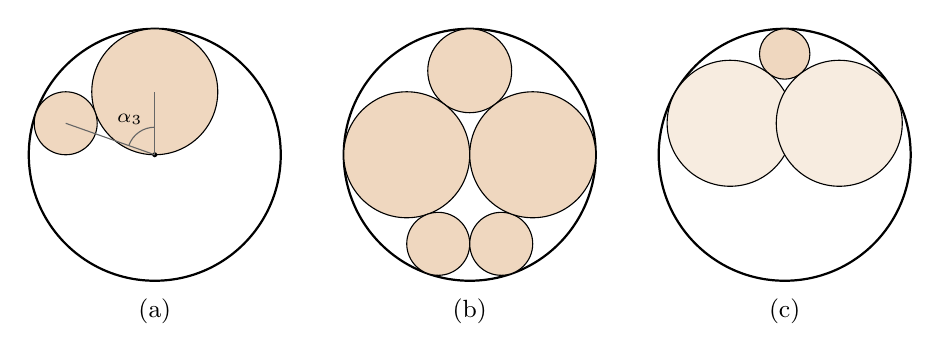
\begin{tikzpicture}
  \begin{scope}[shift={(0,0)}]
\draw[thick] (0,0) circle (1.6);
\draw[fill=copper!25] (0.000,0.800) circle (0.800);
\draw[fill=copper!25] (-1.131,0.400) circle (0.400);
\fill (0,0) circle (0.9pt);
\draw[inkmuted] (0,0) -- (0.000,0.800);
\draw[inkmuted] (0,0) -- (-1.131,0.400);
\draw[inkmuted] (0.000,0.350) arc (90:160.53:0.35);
\node[font=\scriptsize] at (-0.318,0.449) {$\alpha_3$};
\node[below, font=\small] at (0,-1.7000000000000002) {(a)};
\end{scope}
\begin{scope}[shift={(4,0)}]
\draw[thick] (0,0) circle (1.6);
\draw[fill=copper!25] (0.000,1.067) circle (0.533);
\draw[fill=copper!25] (-0.800,0.000) circle (0.800);
\draw[fill=copper!25] (-0.400,-1.131) circle (0.400);
\draw[fill=copper!25] (0.400,-1.131) circle (0.400);
\draw[fill=copper!25] (0.800,-0.000) circle (0.800);
\node[below, font=\small] at (0,-1.7000000000000002) {(b)};
\end{scope}
\begin{scope}[shift={(8,0)}]
\draw[thick] (0,0) circle (1.6);
\draw[fill=copper!25] (0.000,1.280) circle (0.320);
\draw[fill=copper!12] (-0.693,0.400) circle (0.800);
\draw[fill=copper!12] (0.693,0.400) circle (0.800);
\node[below, font=\small] at (0,-1.7000000000000002) {(c)};
\end{scope}

\end{tikzpicture}
\caption{(a) Rim coins $\frac12$ and $\frac14$ subtend $\alpha_3=\arccos\frac13$ at the centre. (b) The asker's $n=4$ ring $\frac13,\frac12,\frac14,\frac14,\frac12$: its angles $\alpha_2+\alpha_3+\alpha_9+\alpha_3+\alpha_2$ add up to $2\pi$. (c) For $n=5$ a $\frac15$ coin on the rim must sit between two half coins at $60^\circ$ each, and then the half coins, $120^\circ$ apart, overlap.}
\label{fig:rim}
\end{figure}

\section{Which relations hold among the angles}

Write $d-1=s^2a$ with $a$ squarefree, and call $a$ the \emph{class} of $d$; put $d=1$, where $\alpha_1=\pi$, in a class of its own. By~\eqref{eq:alpha}, $\tan\frac{\alpha_d}2=1/(s\sqrt a)$, so $\frac{\alpha_d}2=\frac\pi2-\arctan(s\sqrt a)$; since $\arg(1-is\sqrt a)=-\arctan(s\sqrt a)$,
\begin{equation}\label{eq:arg}
\alpha_d=\pi+2\arg\beta_d,\qquad \beta_d=1-s\sqrt{-a}\in\mathbb Q(\sqrt{-a}).
\end{equation}
Two facts decide every relation.

\emph{Splitting.} If $\sum_dm_d\alpha_d$ is a rational multiple of $\pi$ (with $m_d\in\mathbb Z$), then so is the partial sum over each class. This is the Splitting Theorem of Conway, Radin and Sadun~\cite{CRS} for angles whose squared trigonometric functions are rational, which the $\alpha_d$ are.

\emph{Within a class.} Let $K=\mathbb Q(\sqrt{-a})$ and $\gamma=\prod_d\beta_d^{m_d}$. Then $\sum m_d\arg\beta_d$ is a rational multiple of $\pi$ exactly when $\gamma/\bar\gamma$ is a root of unity, that is, when the principal ideals $(\gamma)$ and $(\bar\gamma)$ coincide. Primes of $K$ that are ramified or inert equal their conjugates, so this happens exactly when, for every rational prime $p$ that splits as $\mathfrak p\bar{\mathfrak p}$,
\begin{equation}\label{eq:val}
\sum_dm_d\bigl(v_{\mathfrak p}(\beta_d)-v_{\bar{\mathfrak p}}(\beta_d)\bigr)=0 .
\end{equation}
Each difference is computed from the norm $1+s^2a$ of $\beta_d$: if $p^e$ exactly divides it and $\rho$ is a $p$-adic square root of $-a$, then $v_{\mathfrak p}(\beta_d)=v_p(1-s\rho)$ and $v_{\bar{\mathfrak p}}(\beta_d)=v_p(1+s\rho)$, and these add up to $e$. When~\eqref{eq:val} holds, $2\arg\gamma$ is a multiple of $2\pi/w$, where $w\in\{2,4,6\}$ is the number of roots of unity in $K$; so the class sum is an exact multiple of $\pi/3$ or $\pi/2$, and a floating-point evaluation tells which.

For instance $d=3$ and $d=9$ share the class $a=2$, with $\beta_3=1-\sqrt{-2}$ of norm $3$ and $\beta_9=1-2\sqrt{-2}$ of norm $9$. At the split prime $3$ their valuation differences are $1$ and $-2$, so $2\alpha_3+\alpha_9$ satisfies~\eqref{eq:val}, as the asker's ring requires.

A class containing a single $d$ gives the simplest consequence: then $m_d\alpha_d$ itself must be a rational multiple of $\pi$, and by Niven's theorem, since $\cos\alpha_d$ is rational, this happens only for $d\in\{1,2,4\}$. So \emph{a pair whose $d$ is alone in its class, among the values of $d$ that occur, can never be a rim neighbour pair.}

\begin{proof}[Proof of Theorem~\ref{thm:rim} for $n=5$]
The values of $d$ for $2\le j\le k\le5$ are $1,2,3,4,6,8,9,12,16$, and $6,8,12,16$ are alone in their classes $5,7,11,15$. So none of the pairs $(\frac13,\frac14)$, $(\frac13,\frac15)$, $(\frac14,\frac15)$, $(\frac15,\frac15)$ can be neighbours on the rim, and a $\frac15$ coin must sit between two half coins, at $\alpha_4=60^\circ$ from each. Those two half coins are then $120^\circ$ apart, with centres $2\cdot\frac12\sin60^\circ=\frac{\sqrt3}2<1$ apart, so they overlap (Figure~\ref{fig:rim}(c)).
\end{proof}

\section{All rim arrangements up to $n=1000$}

The same reasoning, done by computer, decides every $n$. Since every multiplicity in~\eqref{eq:sum} is nonnegative, there is a cheap first step.

\emph{Pruning.} In a class, if at some split prime every remaining $d$ with a nonzero valuation difference has the same sign, then~\eqref{eq:val} forces all of them to have multiplicity $0$; remove them and repeat. If some size $\frac1j$ is left with no possible neighbour, there is no rim arrangement.

For $7\le n\le10$ and $20\le n\le1000$ the pruning alone strands some size, for example $\frac17$ for $7\le n\le10$ and $\frac1{20}$ for $20\le n\le27$; the script prints the stranded sizes for each $n$. For the remaining values $n=5,6$ and $11\le n\le19$ an exhaustive search finishes the job:
\begin{enumerate}
\item in each class, list the multiplicity vectors with angle sum at most $2\pi$ that satisfy~\eqref{eq:val}, and their exact values;
\item combine the classes in all ways that give exactly $2\pi$;
\item assign each $d$ to pairs $(j,k)$ with $(j-1)(k-1)=d$, keep the multigraphs on the sizes that use every size and have even degrees, and search their Euler circuits for one in which no two coins overlap.
\end{enumerate}
The search reproduces the known small cases (three cycles for $n=3$, among them the asker's, and exactly the asker's ring for $n=4$) and finds nothing for $5\le n\le22$; at $n=22$ there are $1264$ multisets of angles summing to exactly $2\pi$, and none survives step~3. Every overlap that rejects a candidate does so by a margin of at least $0.05$ in the radius-$1$ scale, far above rounding error, and no search was truncated. This proves Theorem~\ref{thm:rim}.\qed

\section{Coronas and triangulated arrangements}

The bookkeeping works around any coin, not only around the centre of the tray. Let a coin of curvature $m$ touch two bodies $a$ and $b$ that touch each other, where the tray counts as curvature $-1$. The triangle of centres has sides $|\frac1m+\frac1a|$, $|\frac1m+\frac1b|$, $|\frac1a+\frac1b|$, so the angle between the two contact directions has rational cosine $c=p/q$ (with the sign of $c$ reversed when one of the bodies is the tray, whose contact direction points away from its centre). With $q^2-p^2=s^2a$ this angle is $\arg(p+s\sqrt{-a})$, and the splitting and valuation criteria apply unchanged.

A \emph{closed corona} of a coin is a cyclic list of neighbours, each touching the next, with no two overlapping, the tray used at most once, and contact directions turning by exactly $2\pi$. Coronas of this kind, with exact angle relations, are the main tool in the classification of compact packings of the plane by discs of two and three sizes~\cite{Kennedy,FHS}. If the contact graph of an arrangement, tray included, is a triangulation, then every coin has a closed corona, namely its actual neighbours in cyclic order, and the contact graph is connected.

\begin{figure}[ht]
\centering
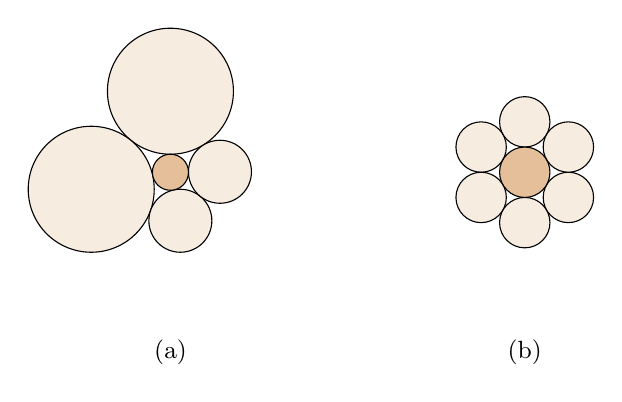
\begin{tikzpicture}
  \begin{scope}[shift={(0,0)}]
\draw[fill=copper!12] (0.000,1.029) circle (0.800);
\draw[fill=copper!12] (-1.006,-0.216) circle (0.800);
\draw[fill=copper!12] (0.126,-0.616) circle (0.400);
\draw[fill=copper!12] (0.629,0.006) circle (0.400);
\draw[fill=copper!40] (0,0) circle (0.229);
\node[below, font=\small] at (0,-2.000) {(a)};
\end{scope}
\begin{scope}[shift={(4.5,0)}]
\draw[fill=copper!12] (0.000,0.640) circle (0.320);
\draw[fill=copper!12] (-0.554,0.320) circle (0.320);
\draw[fill=copper!12] (-0.554,-0.320) circle (0.320);
\draw[fill=copper!12] (-0.000,-0.640) circle (0.320);
\draw[fill=copper!12] (0.554,-0.320) circle (0.320);
\draw[fill=copper!12] (0.554,0.320) circle (0.320);
\draw[fill=copper!40] (0,0) circle (0.320);
\node[below, font=\small] at (0,-2.000) {(b)};
\end{scope}

\end{tikzpicture}
\caption{Two closed coronas. (a) A $\frac17$ coin ringed by $\frac12,\frac12,\frac14,\frac14$: the four angles between consecutive contacts add up to exactly $2\pi$, an identity the valuation test certifies. (b) Six $\frac15$ coins around a $\frac15$ coin, the only closed corona of a $\frac15$ coin when $5\le n\le7$.}
\label{fig:corona}
\end{figure}

\begin{proof}[Proof of Theorem~\ref{thm:tri}]
Let $R$ be the smallest set of sizes containing every size with a closed corona that uses the tray, and every size with a closed corona that uses a size in $R$. In a triangulated arrangement, follow a path of contacts from any coin to the tray; walking it backwards shows that every size present lies in $R$. Computing all closed coronas exactly, with the criteria above, gives the sizes outside $R$:
\begin{center}
\begin{tabular}{lcccccccccccc}
\toprule
$n$ & 5--7 & 8 & 9 & 10, 11 & 12 & 13--16\\
\midrule
not in $R$ & $\frac15$ & $\frac15,\frac18$ & $\frac15,\frac18,\frac19$ & $\frac18,\frac19$ & $\frac19$ & $\frac19,\frac1{13}$\\
\bottomrule
\end{tabular}
\end{center}
So for every $5\le n\le16$ some size cannot occur. The angle relations in this computation are decided exactly; the overlap tests are numerical, but a candidate is rejected only when two coins overlap by more than $10^{-6}$, and every rejection in fact has a margin of at least $0.004$. Near-tangencies are accepted, which can only add coronas and enlarge~$R$, and no search was truncated.
\end{proof}

For $5\le n\le7$, for example, the only closed corona of a $\frac15$ coin is six $\frac15$ coins (Figure~\ref{fig:corona}(b)), so in a triangulated arrangement the $\frac15$ coins would form a region that never reaches the tray. The computation does find other exact coronas, such as a $\frac17$ coin ringed by $\frac12,\frac12,\frac14,\frac14$ (Figure~\ref{fig:corona}(a)), which is the identity behind the asker's near-fit with $\frac12,\frac13,\frac14,\frac16,\frac17$.

\section{Coins in a corner: a congruence}

\begin{proof}[Proof of Proposition~\ref{prop:desc}]
If the tray (curvature $-1$) and coins of curvatures $b,c,k$ are mutually tangent, Descartes' circle theorem holds for the quadruple $(-1,b,c,k)$ of integers, and the Apollonian packing it generates is integral and contains the tray. The theory of root quadruples~\cite{GLMWY} reduces every integral Apollonian packing to a unique root quadruple $(a,b,c,d)$, one with $a<0\le b\le c\le d$ and $a+b+c\ge d$, where $a$ is the curvature of the bounding circle. Here $a=-1$, and $b\ge2$ because every other circle of the packing is smaller than the tray. Put $x=b+c-1$. Descartes' equation $(x+d)^2=2(1+b^2+c^2+d^2)$ rearranges to $(x-d)^2=4(bc-b-c)$, while $0\le x-d\le b-1$ because $c\le d\le x$. Since $c\ge b$, $bc-b-c\ge b^2-2b$, so $4(b^2-2b)\le(b-1)^2$, which forces $b=2$; then $4(c-2)\le1$ gives $c=2$, and $(x-d)^2=0$ gives $d=3$. So the root quadruple is $(-1,2,2,3)$. By the congruence theorem of Graham, Lagarias, Mallows, Wilks and Yan~\cite{GLMWY}, the curvatures in that packing lie in the classes $2,3,6,11,14,15,18,23\pmod{24}$; a direct computation of all its curvatures up to $5000$ agrees.
\end{proof}

So the familiar exact constructions (filling the gap between the tray and two touching coins, Pappus chains, Steiner chains around a central coin, which inversion turns into Descartes quadruples) can never produce a $\frac14$, $\frac15$ or $\frac17$ coin. Every arrangement with $n\ge4$ must lock its $\frac14$ coin some other way; the asker's ring does it with the identity $2\alpha_3+\alpha_9=\pi$.

\begin{remark}[Why searches find near-misses; heuristic]
With $N$ coins there are $2N-1$ degrees of freedom, and a coin placed against two existing bodies uses up exactly its two. Rigidity needs a positive self-stress, which generically needs at least one contact more than the degrees of freedom; a configuration already determined meets an extra tangency only through an algebraic coincidence. So numerical searches produce endless near-packings, and an exact arrangement, if one exists, rests on an identity such as $2\alpha_3+\alpha_9=\pi$. The rim case is exactly where such identities can be classified completely.
\end{remark}

\section{Verification}

The law-of-cosines formula~\eqref{eq:alpha}, the fact that $\alpha_d$ is a rational multiple of $\pi$ only for $d\in\{1,2,4\}$ (from Niven's theorem in Mathlib), the identity $2\alpha_3+\alpha_9=\pi$, the overlap in the $n=5$ argument and the uniqueness of the root quadruple $(-1,2,2,3)$ are proved in Lean~4~\cite{mathlib}. The splitting theorem~\cite{CRS}, the valuation criterion (standard algebraic number theory, as explained in Section~3) and the congruence theorem~\cite{GLMWY} are quoted, and the searches are computations. The valuation criterion is cross-checked against $60$-digit numerics on $122{,}400$ random combinations ($944$ relations, no disagreement), and deleting one prime from the valuation vectors makes that check fail. The rim and corona searches report truncations, the smallest overlap margins and near-tangencies, and planted errors (a numerical relation test with tolerance $10^{-3}$ for the rim, $2\cdot10^{-2}$ for coronas) change their output. Code and Lean files are at~\cite{repo}.

\section*{Acknowledgments}

The question and the arrangements for $n\le4$ are Dan's. The reduction of the rim case to the angles $\alpha_d$ is from the answer~\cite{U}, and the near-miss searches are Matthew House's~\cite{House}. The analysis, the computations and the Lean formalisation were carried out with Claude Opus~5.5 (Anthropic). The author is responsible for the content.

\begin{thebibliography}{9}
\bibitem{MO} Dan, \emph{For what values of $n$ can coins of radius $\frac12,\frac13,\frac14,\dots,\frac1n$ be held rigidly in a circular tray of radius~$1$?}, MathOverflow question 513668 (2026), \url{https://mathoverflow.net/q/513668}; Mathematics Stack Exchange question 4940077 (2024), \url{https://math.stackexchange.com/q/4940077}.
\bibitem{U} user596229, answer to~\cite{MO}, MathOverflow answer 513840 (2026), \url{https://mathoverflow.net/a/513840}.
\bibitem{House} M.~House, answer to~\cite{MO}, MathOverflow answer 513851 (2026), \url{https://mathoverflow.net/a/513851}.
\bibitem{CRS} J.~H.~Conway, C.~Radin and L.~Sadun, \emph{On angles whose squared trigonometric functions are rational}, Discrete Comput. Geom. 22 (1999), 321--332.
\bibitem{FHS} Th.~Fernique, A.~Hashemi and O.~Sizova, \emph{Compact packings of the plane with three sizes of discs}, Discrete Comput. Geom. 66 (2021), 613--635.
\bibitem{GLMWY} R.~L.~Graham, J.~C.~Lagarias, C.~L.~Mallows, A.~R.~Wilks and C.~H.~Yan, \emph{Apollonian circle packings: number theory}, J. Number Theory 100 (2003), 1--45.
\bibitem{Kennedy} T.~Kennedy, \emph{Compact packings of the plane with two sizes of discs}, Discrete Comput. Geom. 35 (2006), 255--267.
\bibitem{mathlib} The mathlib Community, \emph{The Lean mathematical library}, in: Proc. 9th ACM SIGPLAN Int. Conf. on Certified Programs and Proofs (CPP 2020), 367--381.
\bibitem{repo} V.~Jandhyala, code and Lean proofs, \url{https://github.com/jvvk/mathematics/tree/main/coins-in-a-tray}.
\end{thebibliography}

\end{document}
